	\subsection{Теорема Куммера}

	Начнём с вот такой полезной леммы:

	\begin{lemma}\label{ind_and_p}
		Следующие условия равносильны:
		\begin{enumerate}
			\item $p \not\ \mid \ind(\theta)$.
			\item $\Z[\theta]/(p) \to \cO_{K}/(p)$~--- изоморфизм.
		\end{enumerate}
	\end{lemma}

	\begin{proof}
		Это я допишу с записи. 
	\end{proof}

	\begin{theorem}[Куммер]\label{Kummer_theorem} 
		Пусть $K = \Q(\theta)$, $\theta \in \cO_{K}$, а $p$~--- такое простое число, что $p \not \ \mid \ind(\theta)$. Пусть $f$~--- минимальный многочлен $\theta$, причем над полем $\Z/p\Z$ его редукция раскладывается в неприводимыке, как 
		\[
			\overline{f} = \prod_{i} \overline{g_i}^{a_i} \in \F_{p}[t], \ \deg{g_i} = d_i, \ g_i \text{~--- унитальные.}
		\]

		Тогда:
		\vspace{-1mm}
		\begin{enumerate}
			\item Идеалы $\fp_i = (g_i(\theta), p)$~--- все простые идеалы, висящие над простым числом $p$. Причём, они попарно различны. 
			\item $\left\lvert \cO_{K}/\fp_i \right\rvert = p^{d_i}$, а значит, $d_i$~--- степень инерции идеала $\fp_i$.
			\item $p\cO_{K} = \prod \fp_i^{a_i}$, то есть $a_i$ есть индексы ветвления идеалов $\fp_i$.
		\end{enumerate}
 	\end{theorem}
 	\begin{proof}
 		Во-первых, покажем, что $\fp_i$ максимальны. Для этого достаточно проверить, что фактор~--- поле. Дейстивтельно, это простое вычисление: 
 		\[
 			\cO_{K}/\fp_{i} = \cO_{K}/(g_i(\theta), p) = \Z[\theta]/(g_i(\theta), p) \cong \Z[t]/(f(t), p, g_i(t)) \cong \F_{p}[t]/\overline{g_i},
 		\]
 		которое является полем, так как многочлен $g_i$ неприводим над $\F_{p}$. 

 		Теперь покажем, что $\fp_i \neq \fp_j$ при $i \neq j$. Предположим противное. Тогда 
 		\[
 			\fp_i = \fp_j = (g_i(\theta), p, g_j(\theta)).
 		\]

 		Но, $\overline{g_i}$ и $\overline{g_j}$~---- различные неприводимые многлчлены над $\F_p$, а мы можем линейно представить их НОД: 
 		\[
 			\exists \overline{h_i}, \overline{h_j}\colon \overline{h_i} \overline{g_i} + \overline{h_j} \overline{g_j} = \overline{1} \implies h_i g_i + h_j + g_j = 1 + p q(t) \in \Z[t].
 		\]
 		Подставляя в последнее равенство $\theta$, мы получаем, что $1 \in (g_i(\theta), g_j(\theta), p) = \fp_i = \fp_j$, что противоречит тому, что $\fp_i$ и $\fp_{j}$~--- в частнсоти, собственные идеалы. 

 		Теперь провреим, что $d_i$~--- степень инерции. Действительно, 
 		\[
 			\cO_{K}/\fp_i \cong \F_{p}[t]/(\overline{g_i}) \implies \left\lvert \cO_{K}/\fp_i \right\rvert = d_i.
 		\]

 		Из условия теоремы мы знаем, что 
 		\[
 			f(t) = \prod g_{i}(t)^{a_i} + p h(t) \implies 0 = f(\theta) = \prod g_{i}(\theta)^{a_i} + p h(\theta) \implies   \prod g_{i}(\theta)^{a_i} \in p\cO_{K} \implies \prod \fp_{i}^{a_i} \subset p\cO_{K}.
 		\]

 		Отсюда уже видно, что над $p$ не висит никаких других идеалов. Действительно,  
 		\[
 			p\cO_{K} \subset \fq \implies \prod \fp_i^{a_i} \subset \fq \implies \fp_i \subset \fq \implies \fp_i  = \fq.
 		\]
 		Значит, $\prod \fp_i^{a_i} = (p)I$. Из этого следует, что $a_i \ge e_i$. Остается заметить, что 
 		\[
 			\sum a_i e_i = n, \text{ но } \sum a_i e_i \ge \sum e_i d_i = n \implies a_i = e_i \ \forall i.
 		\]


 	\end{proof}

 	Имеет смысл разобрать полезный частный случай этой теоремы: когда  все $a_i$ равны $1$. 

 	\begin{theorem}\label{Criterion_for_Kummer} 
 		Пусть $K = \Q(\theta), \ \theta \in \cO_{K}$, $f$~--- минимальный многочлен $\theta$, а  $p$~--- простое число. Предположим, что 
 		\[
 		 	\overline{f} = \overline{g_1} \cdot \overline{g_2} \cdot \ldots \cdot \overline{g_k} \in \F_{p}[t], \text{ причем}
 		 \] 

 		 $\overline{g_i}$~--- попарно различые и унитальные.  Тогда $p \not \ \mid \ind(\theta)$.
 	\end{theorem}

 	\begin{proof}
 		Рассмотрим идеалы $(p, g_i(\theta)) \subset \cO_{K}$. Пусть $I = (p, g_i(\theta)) = I \subset \Z[\theta]$~--- идеал. Покажем, что $I\cO_{K} \neq \cO_{K}$. Предположим противное и выберем в $\cO_{K}$ целый базис $\omega_1, \ldots, \omega_n$. Тогда мы можем записать каждый элемент базиса с коэффициентами из идеала: 
 		\[
 			\omega_i = \sum a_{i j} \omega_{j}
 		\]
 		Перенося всё в одну часть и обозначая $A = (a_{i j})$, мы имеем такую систему уравнений:
 		\[
 			\lr*{E - A} \cdot \begin{pmatrix} \omega_1 \\ \omega_2 \\ \vdots \\ \omega_n \end{pmatrix} = \begin{pmatrix} 0\\ 0  \\ \vdots \\ 0\end{pmatrix}
 		\]
 		В таком случае $\det{(E - A)} = 0$, из чего следует, что $1 \in I$, а это даёт нам противоречие.

 		Значит, он содержится в некотром максимальном идеале, $(p, g_i(\theta)) \subset \fp_i \subset \cO_{K}$. Теперь нам достаточно показать, что (по лемме \ref{ind_and_p})
 		\[
 		 	\Z[\theta]/(p) \cong \cO_{K}/(p).
 		 \] 
 		 Рассмотрим следующую коммутативную диаграмму: 

 		 \begin{center}
 		 	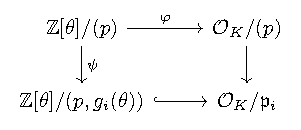
\includegraphics{lectures/4/pictures/cd_1.pdf}
 		 \end{center}

 		 Достаточно проверить, что $\Ker{\varphi} = 0$. Дейстивтельно, пусть $\overline{\alpha} \in \Ker{\varphi}$, тогда $\psi(\overline{\alpha}) = 0$, а значит, $\alpha \in (p, g_{i}(\theta)) \ \forall i$, из чего следует, что 
 		 \[
 		 	\alpha^k \in \prod_{i} (p, g_{i}(\theta)) \in p\Z[\theta] \implies \overline{\alpha}^k = \overline{0} \text{ в } \Z[\theta]/(p),
 		 \]
 		 то есть мы нашли нильпотентный элемент. С другой стороны, 
 		 \[
 		 	\Z[\theta]/(p) \cong \F_{p}[t]/\lr*{\overline{f}}, 
 		 \]
 		 а так как $f$ свободно от квадратов; то, что написано справа~--- прямое произведение полей. Значит, $\overline{\alpha} = 0$  и ядро тривиально. 
 	\end{proof}

 	\begin{example}
 		Посмотрим на конкретное применение теоремы Куммера. Пусть $p \not \ \mid m, \ K = \Q(\zeta_m)$.

 		Как мы знаем, минимальный многочлен первообразного корня степени $m$~--- это круговой многочлен $\Phi_{m}$, $\deg{\Phi_{m}} = \varphi(m)$. Нетрудно заметить, что $\Phi_{m} \not \ \mid x^m - 1$. Заметим, что $\overline{x^m - 1} \in \F_{p}[x]$ имеет попарно различные корни (так как он взимнопрост со своей производной), то есть свободен от квадратов. Тогда $\Phi_{m}$ также свободен от квадратов, а по теореме~\ref{Criterion_for_Kummer} это даёт нам, что $p \not \ \mid \ind\lr*{\theta}$, а это уже даёт нам применять теорему Куммера. Разложим его в неприводимые множители 
 		\[
 			\overline{\Phi_{m}} = \overline{g_1} \cdot \ldots \cdot \overline{g_k}, \ \overline{g_i} \text{~--- попарно различны}.
 		\]

 		Кроме того, как мы знаем,

 		\[
 			\fp \cO_{K} = \fp_1 \fp_2 \cdot \ldots \cdot \fp_{k}, \quad \fp_{i} = (p, g_{i}(\theta)).
 		\]
 		Так как $K/\Q$~---расширение Галуа, нам достаточно найти хоть какую-нибудь степень инерции. 

 		\begin{statement} 
 			Степень инерции идеалов $\fp_i$ есть минимальное число $f$ такое, что $m \mid p^f - 1 $.
 		\end{statement}
 		\begin{proof}
 			Как мы знаем, корни $\overline{x^m - 1}$ образубт циклическую группу. Пусть $\theta$~--- образующая этой группы, $\theta \in \F_{p}^{alg}$. 

 		\[
 			x^m - 1 = \Phi_{m}(x) \cdot \
 		\]

 		\textcolor{red}{Доказательство утверждения надо бы переписать!!!!}

 		Отсюда мы получаем, что $\overline{g_1(\theta)} = 0$.	
 		\end{proof}

 		\begin{homework}
 			Задачи:
 			\begin{enumerate}
 				\item Рассмотрим кубическое расщирение $K = \Q(\sqrt[3]{15}) = \Q(\rho)$. 

 				0) Посчитать кольцо $\cO_{K}$.

 				а) Вычислить $\Nm(\rho), \ \Nm(\rho - 1), \ \Nm(\rho + 1), \Nm(\rho - 3)$.

 				б) Докажите, что над простым числом 3 лежит ровно один простой идеал $\rho_3$.

 				в) Докажите, что $\rho_3$~--- главный. Найдите его образующую с помощью разложений $(\rho - 3)$ и $(\rho + 3)$.

 				г) Докажите, что $\frac{9(\rho + 1)^3}{(\rho  - 3)^6}  \in \cO_{K}^{*}$. 

 				\item Вычислить $\cO_{K},$ где $K = \Q(\sqrt{p_1}, \ldots, \sqrt{p_k})$, если $p_i$~--- простые и $p_i \equiv 1 \pmod{4}$.
 				\item  Доказать, что $\upsilon_{\fp}(\cD) \ge e - 1$, где $ e = e(\fp)$~--- индекс ветвления. 

 			\end{enumerate}
 		\end{homework}

 		
 	\end{example}
